\chapter{Design Of 16x16 Vedic Multiplier}

\indent\indent The Verilog code and the testbench are written for a 16x16 Vedic multiplier using a carry-save adder and high-speed area efficient adder.


\section{Verilog Code and Testbench for 16x16 Vedic Multiplier}
Figure ~\ref{fig:x1} illustrates the steps to multiply two 2-bit numbers. Converting the above figure to a hardware equivalent we have 3 and gates that will act as 2-bit multipliers and two half adders to add the products to get the final product. Here is the hardware detail of the multiplier.
\begin{figure}[htb]
	\centering
	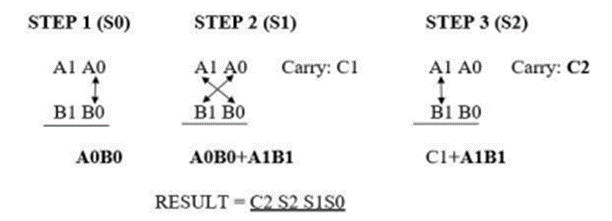
\includegraphics[width=0.80\columnwidth]{Figures/x1}	
	\caption{Steps to Multiply 2x2 Vedic Multiplier}
	\label{fig:x1}
\end{figure}
Where "a" and "b" are two numbers to be multiplied and "q" is the product. With this design we are now ready to code this in verilog easily using and gates and HA (half adders). To make the design more modular we try to write code for HA first and then instantiate it to have the final product. \\
\begin{figure}[htb]
	\centering
	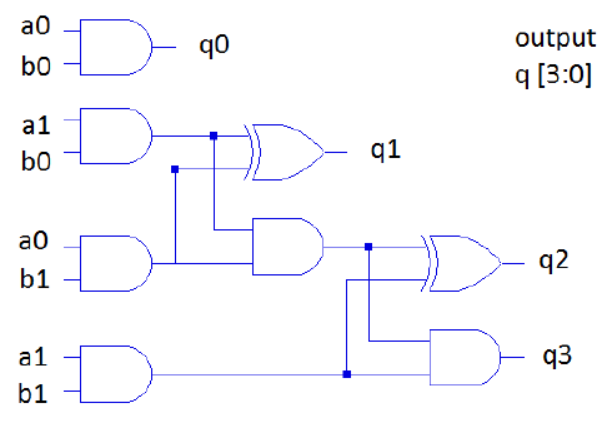
\includegraphics[width=0.5\columnwidth]{Figures/x6}	
	\caption{Design of 2x2 Vedic Multiplier}
	\label{fig:x6}
\end{figure}
The Verilog code for 2x2 Vedic Multiplier is \\
`timescale 1ns / 1ps\\
//////////////////////////////////////////////////////////////////////////////////\\
// Company: \\
// Engineer: \\
// \\
// Create Date:    12:34:18 08/01/2013 \\
// Design Name: \\
// Module Name:    vedic\_2\_x\_2 \\
// Project Name: \\
// Target Devices: \\
// Tool versions: \\
// Description: \\
//
// Dependencies: \\
//
// Revision: \\
// Revision 0.01 - File Created \\
// Additional Comments: \\
//\\
//////////////////////////////////////////////////////////////////////////////////\\
module vedic\_2\_x\_2(\\
a,\\
b,\\
c\\
    );\\
input [1:0]a;\\
input [1:0]b;\\
output [3:0]c;\\
wire [3:0]c;\\
wire [3:0]temp;\\
//stage 1\\
// four multiplication operation of bits according to vedic logic done using and gates \\
assign c[0]=a[0]\&b[0]; \\
assign temp[0]=a[1]\&b[0];\\
assign temp[1]=a[0]\&b[1];\\
assign temp[2]=a[1]\&b[1];\\
//stage two \\
// using two half adders \\
ha z1(temp[0],temp[1],c[1],temp[3]);\\
ha z2(temp[2],temp[3],c[2],c[3]);\\
endmodule\\
\\
The Verilog code for 4x4 Vedic Multiplier is\\
`timescale 1ns / 1ps\\
//////////////////////////////////////////////////////////////////////////////////\\
// Company: \\
// Engineer: \\
// \\
// Create Date:    14:30:08 08/01/2013 \\
// Design Name: \\
// Module Name:    vedic\_4\_x\_4 \\
// Project Name: \\
// Target Devices: \\
// Tool versions: \\
// Description: \\
//\\
// Dependencies: \\
//\\
// Revision: \\
// Revision 0$ \cdot $01 - File Created\\
// Additional Comments: \\
//\\
//////////////////////////////////////////////////////////////////////////////////\\
module vedic\_4\_x\_4(\\
a,b,c\\
    );\\
input [3:0]a;\\
input [3:0]b;\\
output [7:0]c;\\
\\
wire [3:0]q0;	\\
wire [3:0]q1;	\\
wire [3:0]q2;\\
wire [3:0]q3;	\\
wire [7:0]c;\\
wire [3:0]temp1;\\
wire [5:0]temp2;\\
wire [5:0]temp3;\\
wire [5:0]temp4;\\
wire [3:0]q4;\\
wire [5:0]q5;\\
wire [5:0]q6;\\
// using 4 2x2 multipliers\\
vedic\_2\_x\_2 z1(a[1:0],b[1:0],q0[3:0]);\\
vedic\_2\_x\_2 z2(a[3:2],b[1:0],q1[3:0]);\\
vedic\_2\_x\_2 z3(a[1:0],b[3:2],q2[3:0]);\\
vedic\_2\_x\_2 z4(a[3:2],b[3:2],q3[3:0]);\\
// stage 1 adders \\
assign temp1 ={2'b0,q0[3:2]};\\
add\_4\_bit z5(q1[3:0],temp1,q4);\\
assign temp2 ={2'b0,q2[3:0]};\\
assign temp3 ={q3[3:0],2'b0};\\
add\_6\_bit z6(temp2,temp3,q5);\\
assign temp4={2'b0,q4[3:0]};\\
// stage 2 adder \\
add\_6\_bit z7(temp4,q5,q6);\\
// fnal output assignment \\
assign c[1:0]=q0[1:0];\\
assign c[7:2]=q6[5:0];\\
\\
endmodule\\
\\
The Verilog code for 8x8 Vedic Multiplier is\\
\\
`timescale 1ns / 1ps \\
//////////////////////////////////////////////////////////////////////////////////\\
// Company: \\
// Engineer: \\
// \\
// Create Date:    15:22:39 08/01/2013 \\
// Design Name: \\
// Module Name:    vedic\_8X8 \\
// Project Name: \\
// Target Devices: \\
// Tool versions: \\
// Description: \\
//\\
// Dependencies: \\
//\\
// Revision: \\
// Revision 0.01 - File Created\\
// Additional Comments: \\
//\\
//////////////////////////////////////////////////////////////////////////////////\\
module vedic\_8X8(a,b,c\\
    );\\
   \\
input [7:0]a;\\
input [7:0]b;\\
output [15:0]c;\\
\\
wire [15:0]q0;	\\
wire [15:0]q1;	\\
wire [15:0]q2;\\
wire [15:0]q3;	\\
wire [15:0]c;\\
wire [7:0]temp1;\\
wire [11:0]temp2;\\
wire [11:0]temp3;\\
wire [11:0]temp4;\\
wire [7:0]q4;\\
wire [11:0]q5;\\
wire [11:0]q6;\\
// using 4 4x4 multipliers\\
vedic\_4\_x\_4 z1(a[3:0],b[3:0],q0[15:0]);\\
vedic\_4\_x\_4 z2(a[7:4],b[3:0],q1[15:0]);\\
vedic\_4\_x\_4 z3(a[3:0],b[7:4],q2[15:0]);\\
vedic\_4\_x\_4 z4(a[7:4],b[7:4],q3[15:0]);\\
\\
// stage 1 adders \\
assign temp1 ={4'b0,q0[7:4]};\\
add\_8\_bit z5(q1[7:0],temp1,q4);\\
assign temp2 ={4'b0,q2[7:0]};\\
assign temp3 ={q3[7:0],4'b0};\\
add\_12\_bit z6(temp2,temp3,q5);\\
assign temp4={4'b0,q4[7:0]};\\
// stage 2 adder\\
add\_12\_bit z7(temp4,q5,q6);\\
// fnal output assignment \\
assign c[3:0]=q0[3:0];\\
assign c[15:4]=q6[11:0];\\
\\
endmodule\\
\\
The Verilog code for 16x16 Vedic Multiplier is\\
\\
`timescale 1ns / 1ps\
//////////////////////////////////////////////////////////////////////////////////\\
// Company: \\
// Engineer: \\
// \\
// Create Date:    15:45:52 08/01/2013 \\
// Design Name: \\
// Module Name:    vedic\_16x16 \\
// Project Name: \\
// Target Devices: \\
// Tool versions: \\
// Description: \\
//\\
// Dependencies: \\
//\\
// Revision: \\
// Revision 0.01 - File Created\\
// Additional Comments: \\
//\\
//////////////////////////////////////////////////////////////////////////////////\\
module vedic\_16x16(a,b,c\\
    );\\
input [15:0]a;\\
input [15:0]b;\\
output [31:0]c;\\
\\
wire [15:0]q0;	\\
wire [15:0]q1;	\\
wire [15:0]q2;\\
wire [15:0]q3;	\\
wire [31:0]c;\\
wire [15:0]temp1;\\
wire [23:0]temp2;\\
wire [23:0]temp3;\\
wire [23:0]temp4;\\
wire [15:0]q4;\\
wire [23:0]q5;\\
wire [23:0]q6;\\
// using 4 8x8 multipliers\\
vedic\_8X8 z1(a[7:0],b[7:0],q0[15:0]);\\
vedic\_8X8 z2(a[15:8],b[7:0],q1[15:0]);\\
vedic\_8X8 z3(a[7:0],b[15:8],q2[15:0]);\\
vedic\_8X8 z4(a[15:8],b[15:8],q3[15:0]);\\
\\
// stage 1 adders \\
assign temp1 ={8'b0,q0[15:8]};\\
add\_16\_bit z5(q1[15:0],temp1,q4);\\
assign temp2 ={8'b0,q2[15:0]};\\
assign temp3 ={q3[15:0],8'b0};\\
add\_24\_bit z6(temp2,temp3,q5);\\
assign temp4={8'b0,q4[15:0]};\\
\\
//stage 2 adder\\
add\_24\_bit z7(temp4,q5,q6);\\
// final output assignment \\
assign c[7:0]=q0[7:0];\\
assign c[31:8]=q6[23:0];\\
\\
endmodule\\
\\
The Verilog Tesbench code for 16x16 Vedic Multiplier is\\
\\
`timescale 1ns / 1ps\\
\\
////////////////////////////////////////////////////////////////////////////////\\
// Company: \\
// Engineer:\\
//\\
// Create Date:   16:15:22 08/01/2013\\
// Design Name:   vedic\_16x16\\
// Module Name:   D:/lfsr/test\_vedic\_16 $ \cdot $ v\\
// Project Name:  lfsr\\
// Target Device:  \\
// Tool versions:  \\
// Description: \\
//\\
// Verilog Test Fixture created by ISE for module:\\ vedic\_16x16\\
//\\
// Dependencies:\\
// \\
// Revision:\\
// Revision 0$ \cdot $01 - File Created\\
// Additional Comments:\\
// \\
////////////////////////////////////////////////////////////////////////////////\\
\\
module test\_vedic\_16;\\
\\
	// Inputs\\
	reg [15:0] a;\\
	reg [15:0] b;\\
\\
	// Outputs\\
	wire [31:0] c;\\
\\
	// Instantiate the Unit Under Test (UUT)\\
	vedic\_16x16 uut (\\
		$ \cdot $a(a), \\
		$ \cdot $b(b), \\
		$ \cdot $c(c)\\
	);\\
\\
	initial begin\\
		// Initialize Inputs\\
		a = 0;\\
		b = 0;\\
		\# 100;\\
		\\
		a = 16'd12;\\
		b = 16'd12;\\
		\# 100;\\
		\\
		a = 16'd15;\\
		b = 16'd13;\\
		\# 100;\\
		\\
		a = 16'd24;\\
		b = 16'd2;\\
		\# 100;\\
		\\
		a = 16'd200;\\
		b = 16'd21;\\
		\# 100;\\
		\\
		a = 16'd36;\\
		b = 16'd48;\\
		\# 100;\\
        \\
		\\
\\
	end\\
      \\
endmodule\\
\\





